\chapter{Problem modelling and implementation}
\label{chap:model}


In this chapter, we are going to formulate our problem using the frameworks that we saw in \autoref{chap:RL}: we will define the basic elements, and then we will develop the formulas and the algorithm that we need to solve it.


\section{The mathematical model}

After a fault occurs and after the technician, together with the remote control room\index{remote control room}, restricts it to a limited number of non-remotely-controlled substations, the problem consists in visiting, and thus reconnecting, these substations in an order that minimizes the cost of the fault. We define the \emph{cost of the fault}\index{cost of the fault} as the amount of time each underlying user of each substation remains disconnected.

Thus, we are given a set of initially disconnected substations $\mathcal C$, with cardinality $|\mathcal C| = N$, between two remotely controlled substations, where these last ones will not be included in the set, since they are already reconnected. Looking at the electrical diagram\index{electrical diagram} of Trieste's power grid, we notice that the number of substations between two remotely controlled ones is always less than $20$, so we can say that in our problem $N < 20$. Luckily, this restricts the dimension of the problem.

\subsection{Elements of the POMDP}

Given that we don't know the position of the fault, but we have to find it while we reconnect the substations, we cannot use an \acrshort{mdp} to model this problem; instead, we will use a \acrshort{pomdp}. The \emph{agent}\index{agent} is the technician that has to decide which substation to visit at each step, while the \emph{environment}\index{environment} includes everything else, among which the possible positions of the fault, and the set of disconnected substations, and their positions and distances.

We define the \emph{state}\index{state} $s$ of the environment as the tuple
\begin{equation}
    s = (x_g, v_k, \{v\})
\end{equation}
where $x_g$ is the position of the fault, $v_k \in \mathcal C$ is the substation at which the technician is currently located, and $\{v\}$ is the set of substations still disconnected after the technician operates in the current substation $v_k$. The set $\{v\}$ can also be chosen to be the set of substations already reconnected, since they are complementary with respect to the set $|\mathcal C|$, but we chose to use the disconnected substations to ease the notation. Since the position of the fault is unknown, the variable $x_g$ is \emph{hidden}, while the variables $v_k$ and $\{v\}$ are \emph{observable}. When the fault occurs, the technician can be everywhere: at home if it happens in the middle of the night, at the company, or on the go. So we introduce an extra dummy substation, called substation $0$, which is the position of the technician when the fault occurs. Given this, we have that the \emph{initial state} is always of the form $s_0 = (x_g, 0, \mathcal C)$, thus we have different initial states, one for every possible position of the fault. Instead, a \emph{terminal state} is of the form $s_t = (x_g, v_k, \varnothing)$. If the fault is localized on an electrical cable, then $v_k$ is one of the two substations at the ends of that faulty cable, so we have two different terminal states; while if the fault is in a substation, $v_k$ is that exact substation, so the terminal state is only one. We notice that the initial cost has a random component, which depends on the position of the technician when the fault occurs, so on the position of the substation $0$. To remove this randomness, we could also impose that the technician position is always at the company, but we chose not to do that, in order to be closer to what really happens.

We then define the \emph{observation}\index{observation} $o$ that the agent senses from the environment as
\begin{equation}
    o = (v_k, \{v\}) \, ,
\end{equation}
and we will also write the state as $s=(x_g, o)$, where $o = (v_k, \{v\})$ is the observation itself. We define the observable $o$ to be a function of $s$:
\begin{equation}
    \begin{array}{cccc}
    o(s): & \mathcal S                                     & \rightarrow & \mathcal O       \\
          & s = (x_g, \, o = \left( v_k, \{v\} \right) \,) & \mapsto     & o = (v_k, \{v\})
\end{array} \, .
\end{equation}
For different states $s = (x_g, \, o = \left( v_k, \{v\} \right) \,)$ that differ only by the position of the fault $x_g$, this function associates the same observable $o = (v_k, \{v\})$. Thus, we have that $o$ is an equivalence class for $s$. For brevity, we will often keep this dependency implicit, and write simply $o$ instead of $o(s)$, meaning that $o = o(s)$. In particular, the observation of an initial state $s_0 = (x_g, 0, \mathcal C)$ is $o_0 = (0, \mathcal C)$.

We define the \emph{action}\index{action} $a$ that the agent can do as the choice of the specific substation the technician will visit as the next step, thus we have that $a \in \mathcal A = \mathcal C$. Actually, since the technician visits only disconnected substations, and never visits already visited substations, we have that $a \in \{v\}$, if we are in state $s = (x_g, v_k, \{v\})$. Thus, we have that the set of available actions depends on the current state:
\begin{equation}
    a \in \mathcal A \big( s = (x_g, v_k, \{v\}) \big) = \{v\} \, .
\end{equation}

We said that this is a problem with terminal states, which occur when we reconnect all the substations. A terminal state will always be reached, since with every action we visit a substation and can reconnect it, so at the very least we remove that substation from the set of disconnected substations. Actually, if we are lucky, each time we can remove half of the substations from the set of disconnected substations. We are therefore positive that the process terminates. So, for this specific problem, it doesn't make sense to introduce a discount factor $\gamma$ (therefore, we have that $\gamma = 1$ in the formulas of \autoref{chap:RL}).

Given all that, we have that the \emph{next state}\index{next-state} $s'$ of the environment is
\begin{equation}
    s' = (x_g, v_{k+1} = a, \{v'\}),
\end{equation}
where $\{v'\}$ is the set of disconnected substations after the technician operates in the substation $v_{k+1}$. Since the technician can always at least reconnect the substation they visit, the set of disconnected substations decreases after each action, so we have that $\{v'\} \subseteq \{v\} \backslash a$.

Finally, we define the \emph{expected reward}\index{expected reward} as the \emph{cost} of going to a certain substation (as the time, in seconds, it takes to go there from where the technician is) multiplied by the number of disconnected users. Let's define as $d_{v_k, v_{k+1}}$ the time in seconds to go from the substation $v_k$ to the next substation $v_{k+1}$, and as $n_{k}$ the number of users still disconnected \emph{before} operating in the substation $v_{k+1}$. So if we are in a state $s = (x_g, v_k, \{v\})$, we make an action $a$, and we end up in a state $s' = (x_g, v_{k+1} = a, \{v'\})$, we have that the number of disconnected users is
\begin{equation}
    n_{k} = \sum_{v \in \{v\}} u_v,
\end{equation}
where $u_v$ is the number of users underneath the substation $v$. So the expected reward has the following formula:
\begin{equation}
    r(s, a, s') = d_{v_k, a} \cdot n_{k} = d_{v_k, a} \cdot \sum_{v \in \{v\}} u_v \, ,
    \label{eq:expected-reward}
\end{equation}
even if it actually depends only on the previous state $s$ and the action taken $a$, but we will keep the term $s'$ to be consistent with the formulas of \cite{SuttonBarto}.
For now, in the cost we will ignore the cost of establishing if the fault is before or after the substation in which the technician is, which is complicated and might raise the total cost significantly. This is because we cannot properly model these costs, due to a lack of data on them. To improve the computation of the cost, we need to carefully take note of the operations the technicians perform when a fault occurs, and then expand the model. To carry out the data collection, one possibility is to implement a serverless Telegram bot using \acrshort{aws}.

In \autoref{fig:sequence-substations} we can see (part of) a trajectory (we miss the rewards) of our \acrshort{pomdp}, using a set of fictional substations.

\begin{figure}[!pht]
    \centering
    \begin{tabular}{cc}
        \subcaptionbox{
            A fault has occurred in $2 \mhyphen 3$. We are in substation $0$ and all the substations are disconnected (orange). Initial state: $s_0 = (2 \mhyphen 3, 0, \mathcal C = \{1,2,3,4,5\})$.
            \label{1} }
            {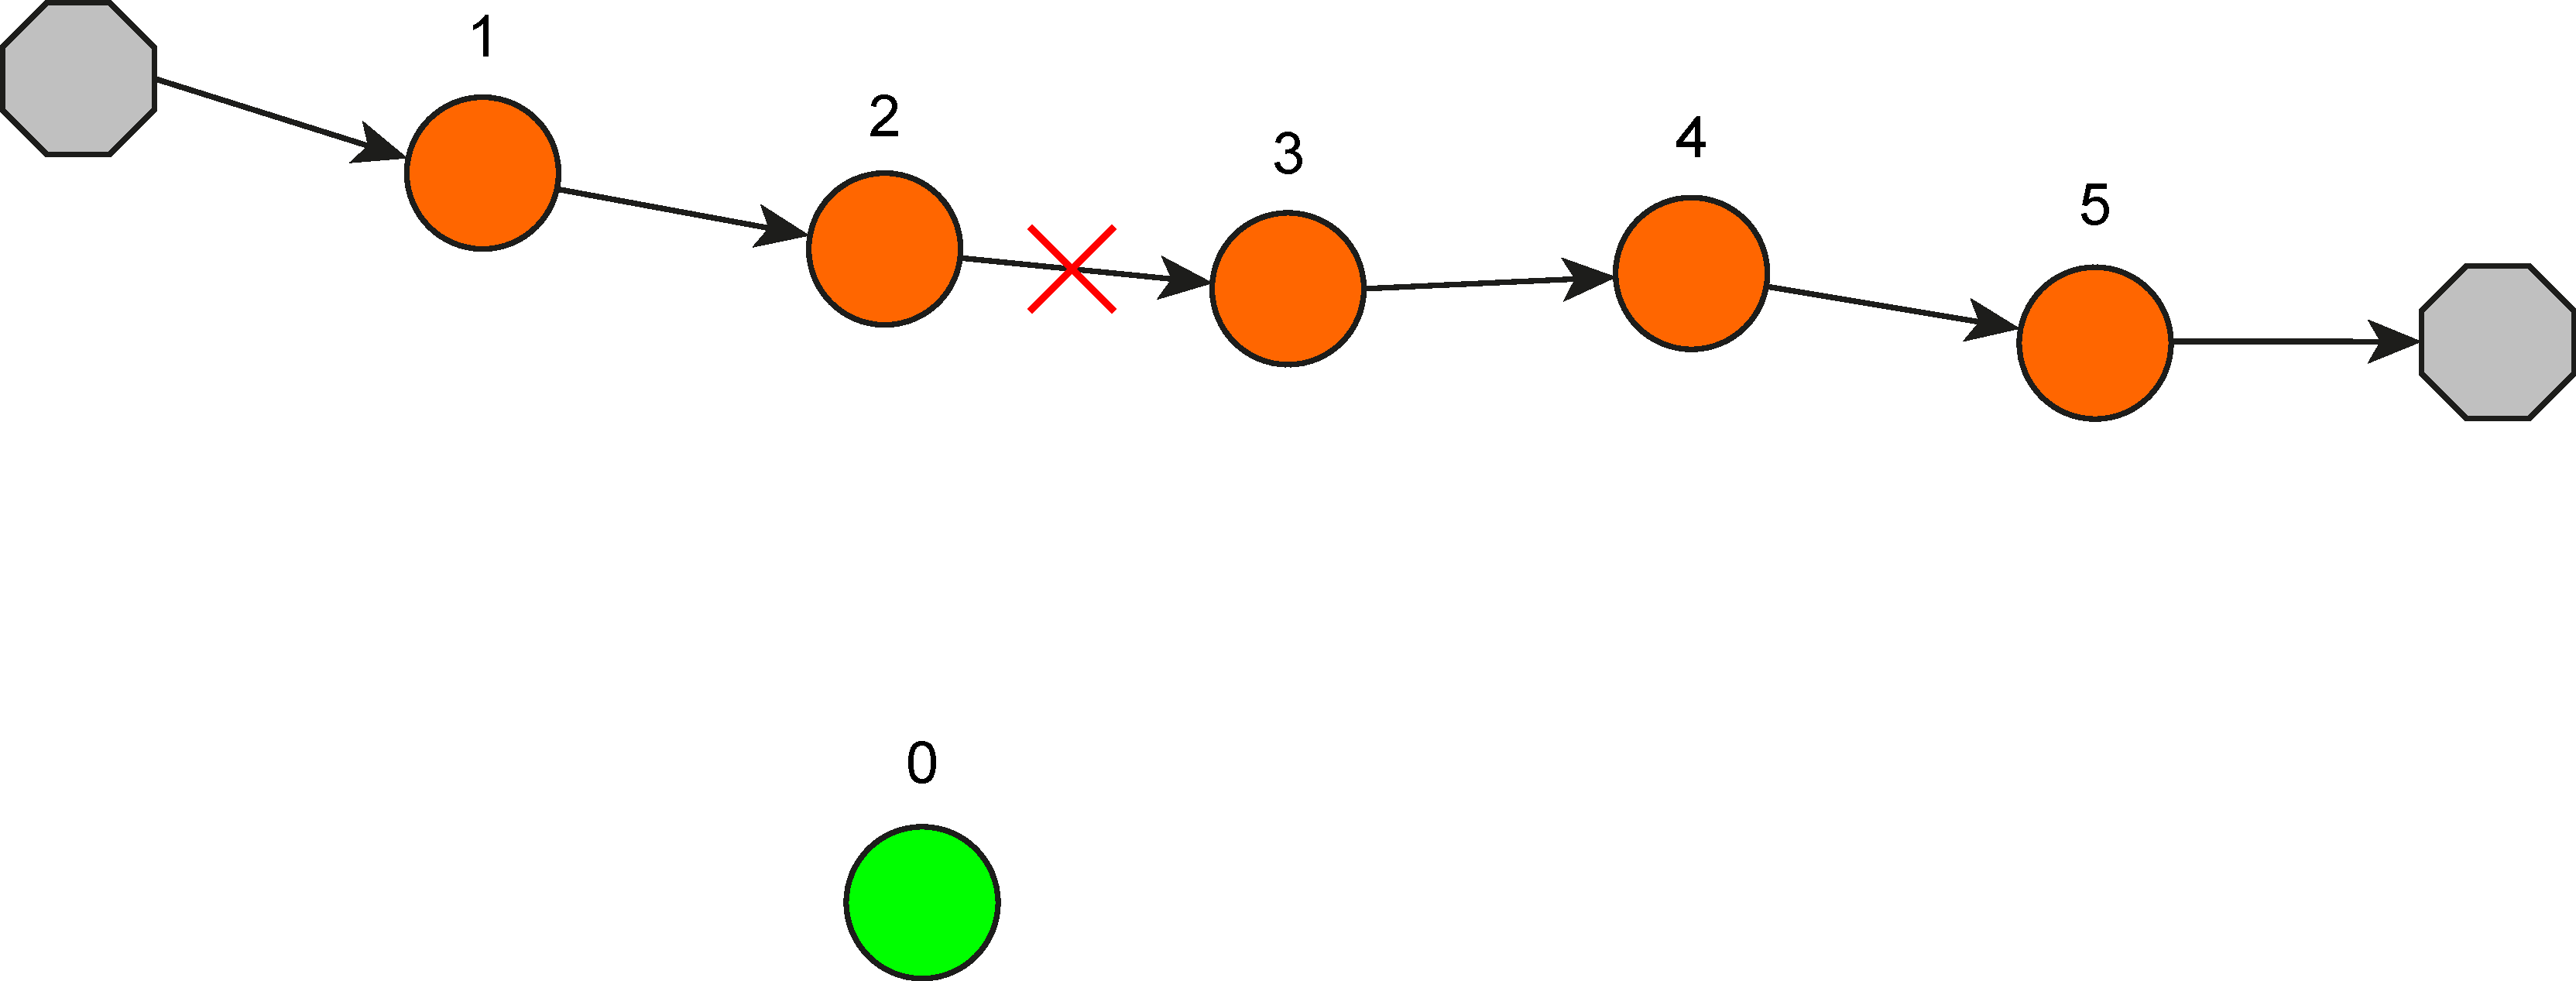
\includegraphics[width=0.45\textwidth,valign=b]{chapters/figures/POMDP_0.pdf}} &
        \subcaptionbox{
            We visit substation $4$ (yellow).\\ Action: $a_0 = 4$.
            \label{2}}
            {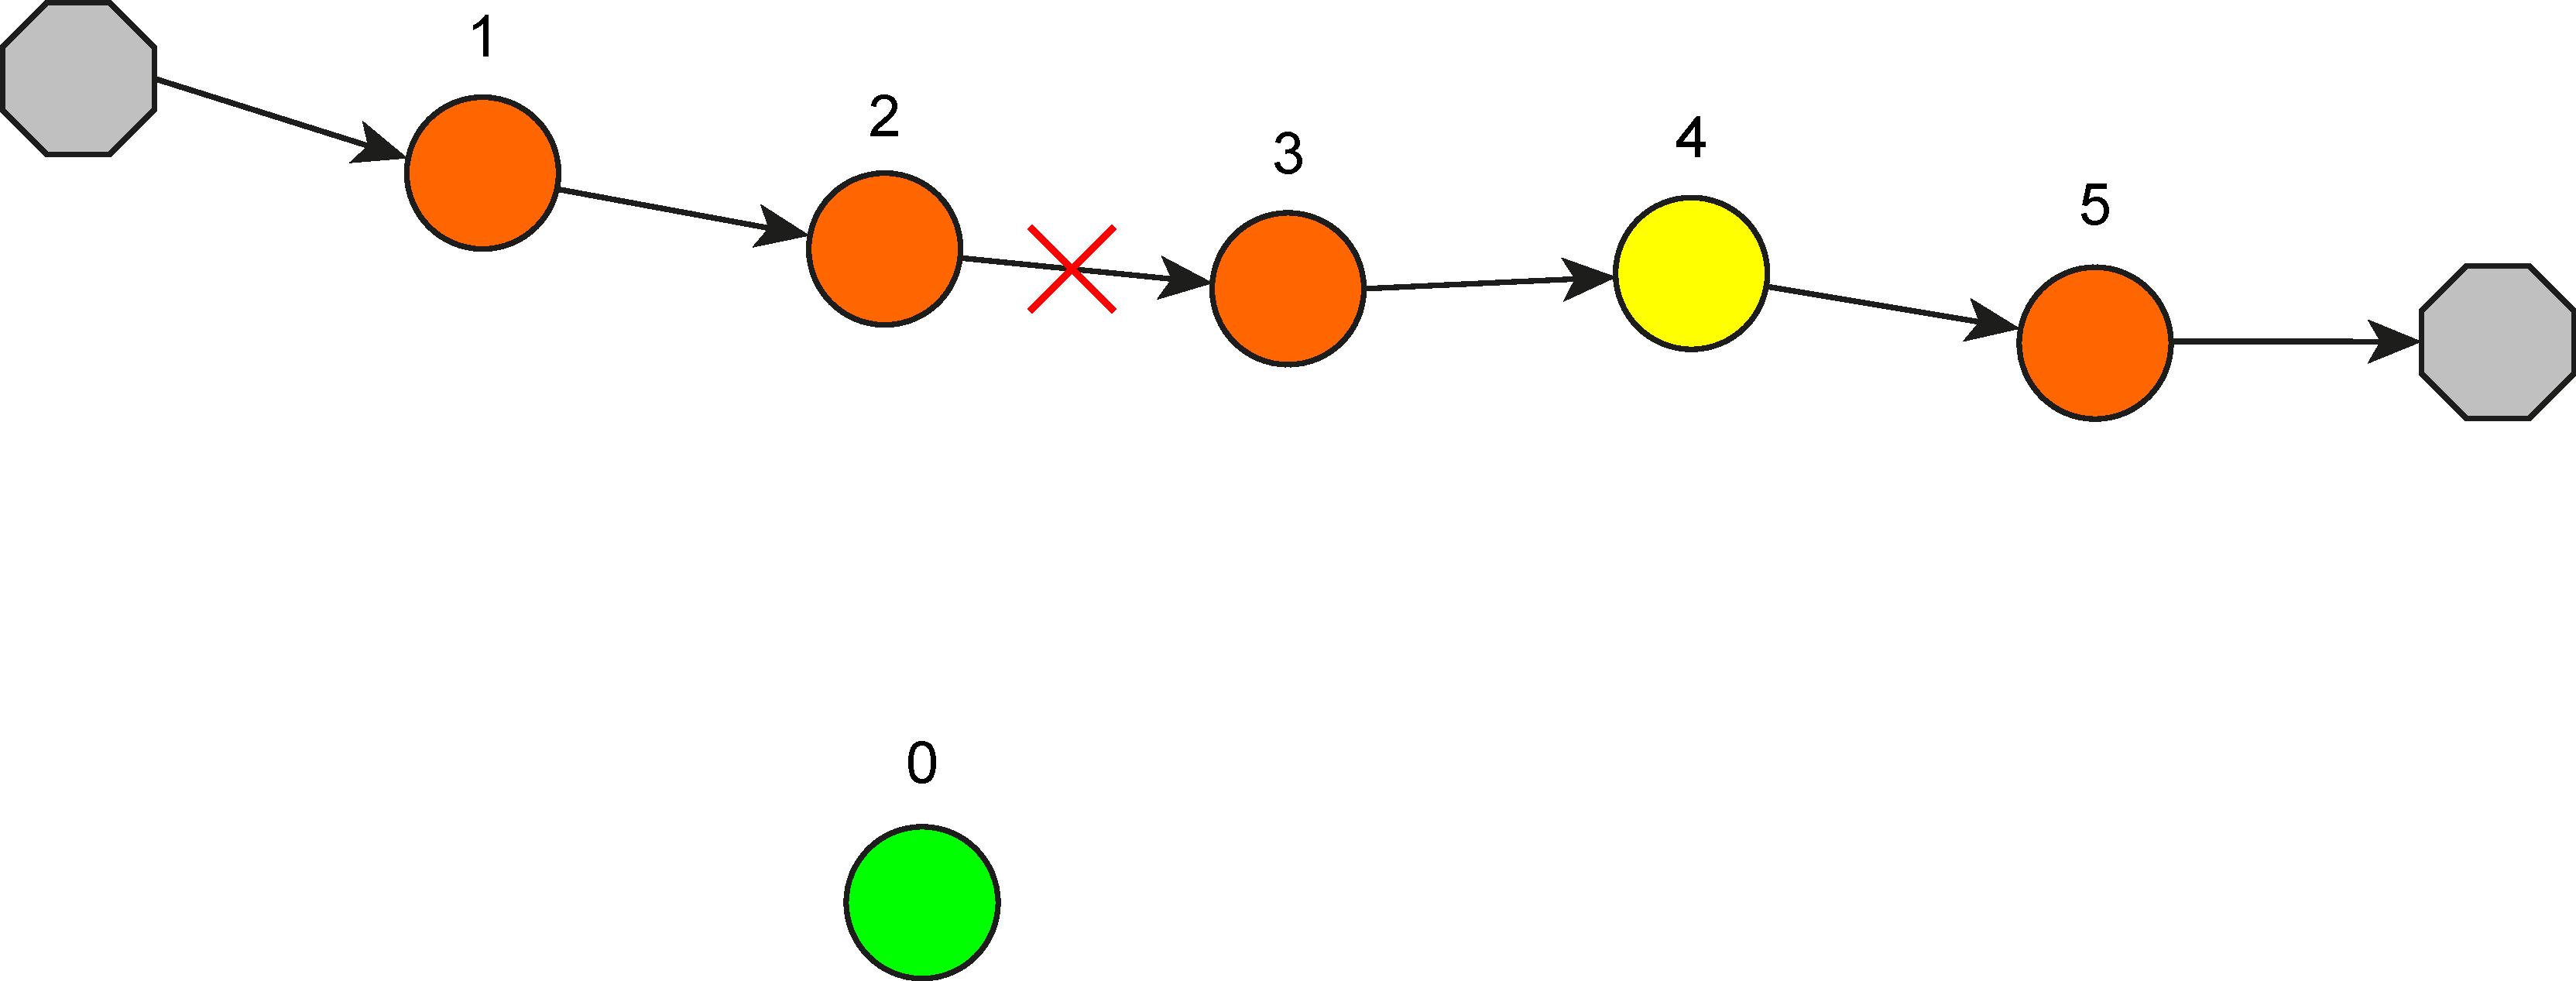
\includegraphics[width=0.45\textwidth,valign=b]{chapters/figures/POMDP_1.pdf}}\medskip\\
        \subcaptionbox{
            We reconnect substations $4$ and $5$ (green). State: $s_1 = (2 \mhyphen 3, 4, \{1,2,3\})$.
            \label{3}}
            {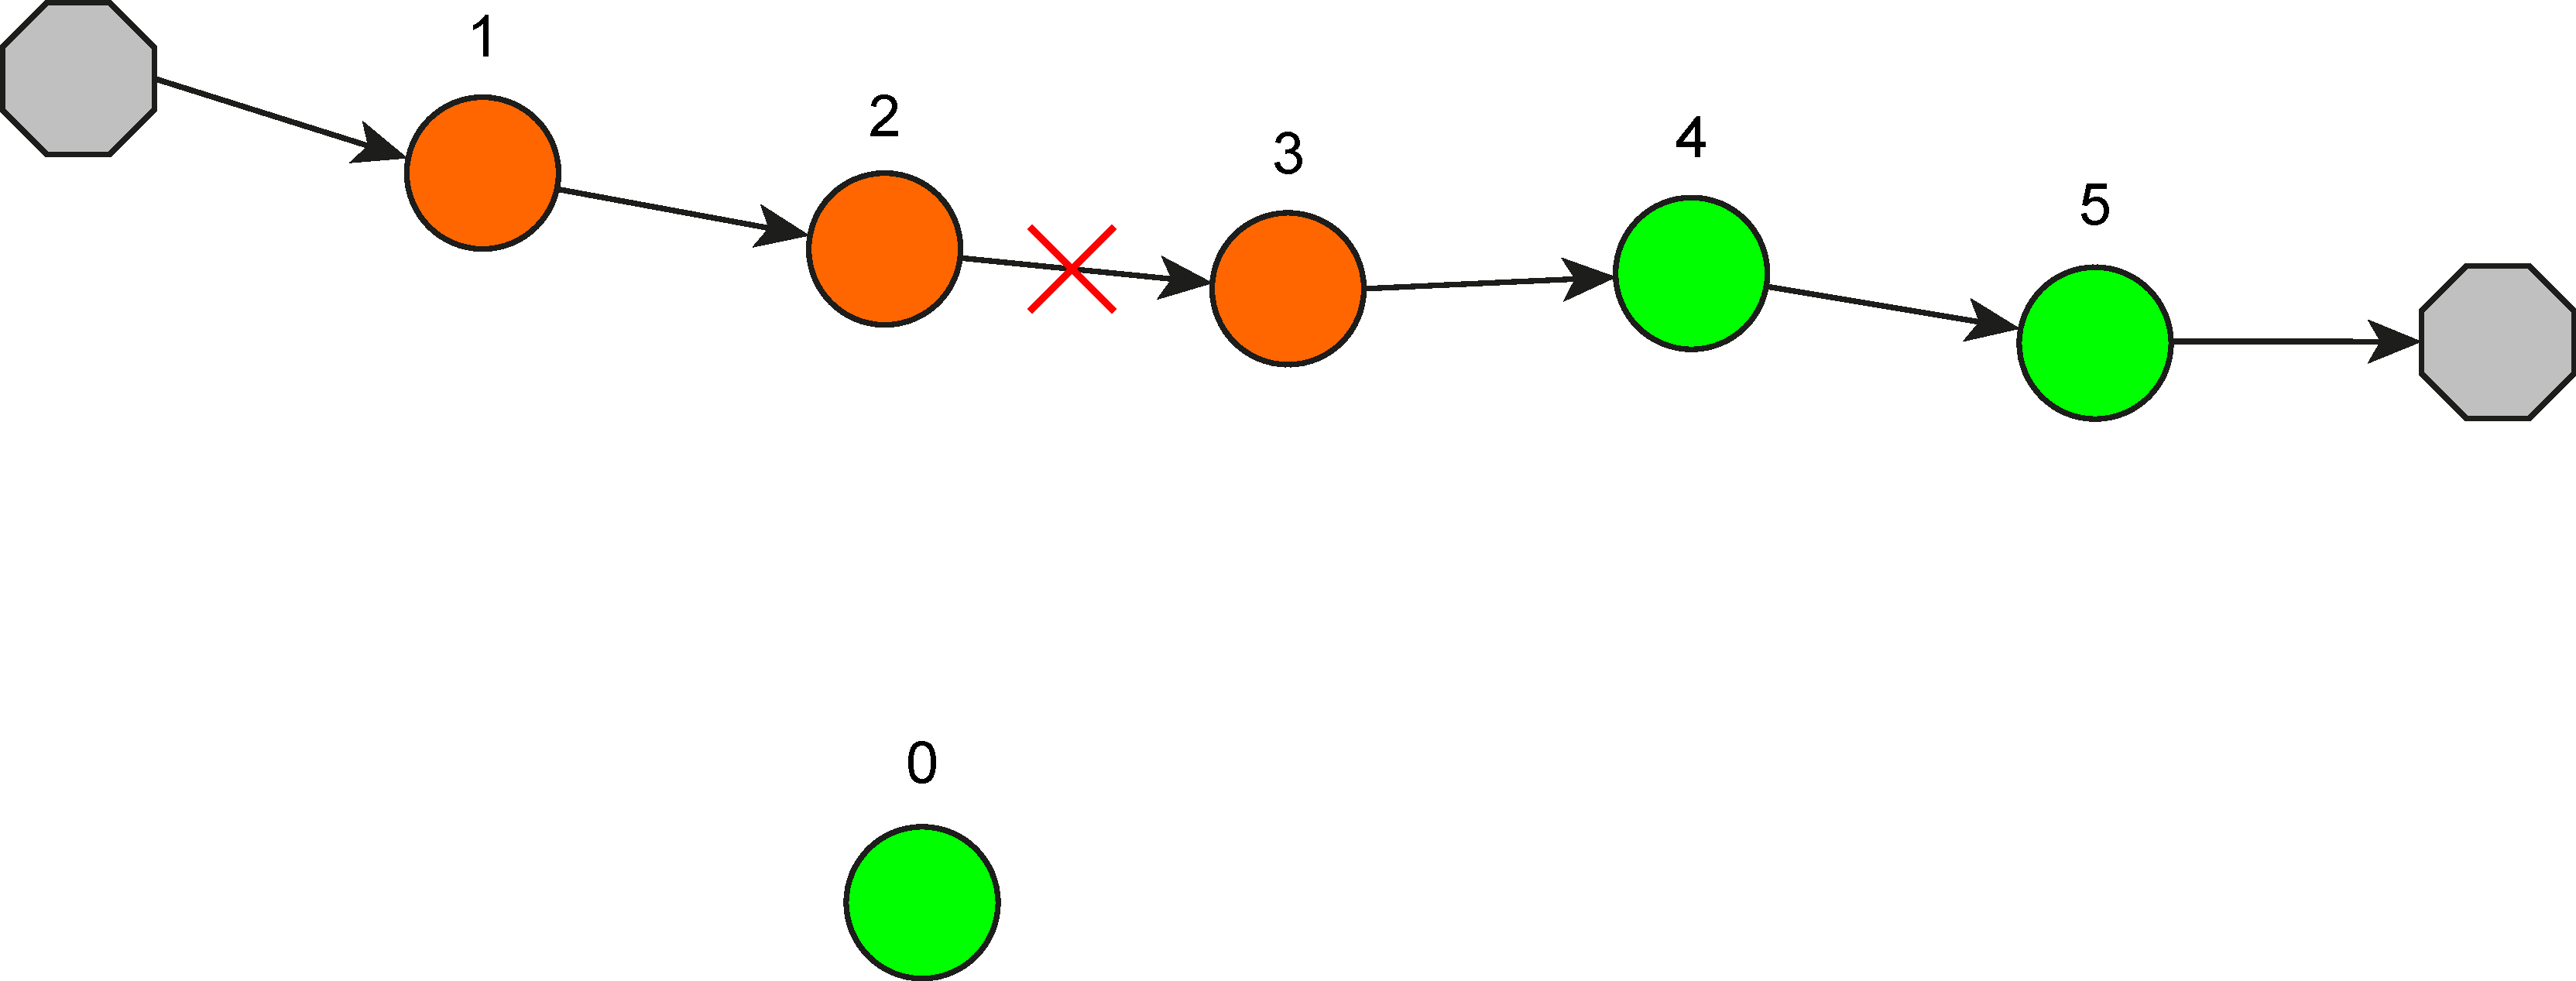
\includegraphics[width=0.45\textwidth,valign=b]{chapters/figures/POMDP_2.pdf}} &
        \subcaptionbox{
            We visit substation $3$ (yellow).\\ Action: $a_1 = 3$.
            \label{4}}
            {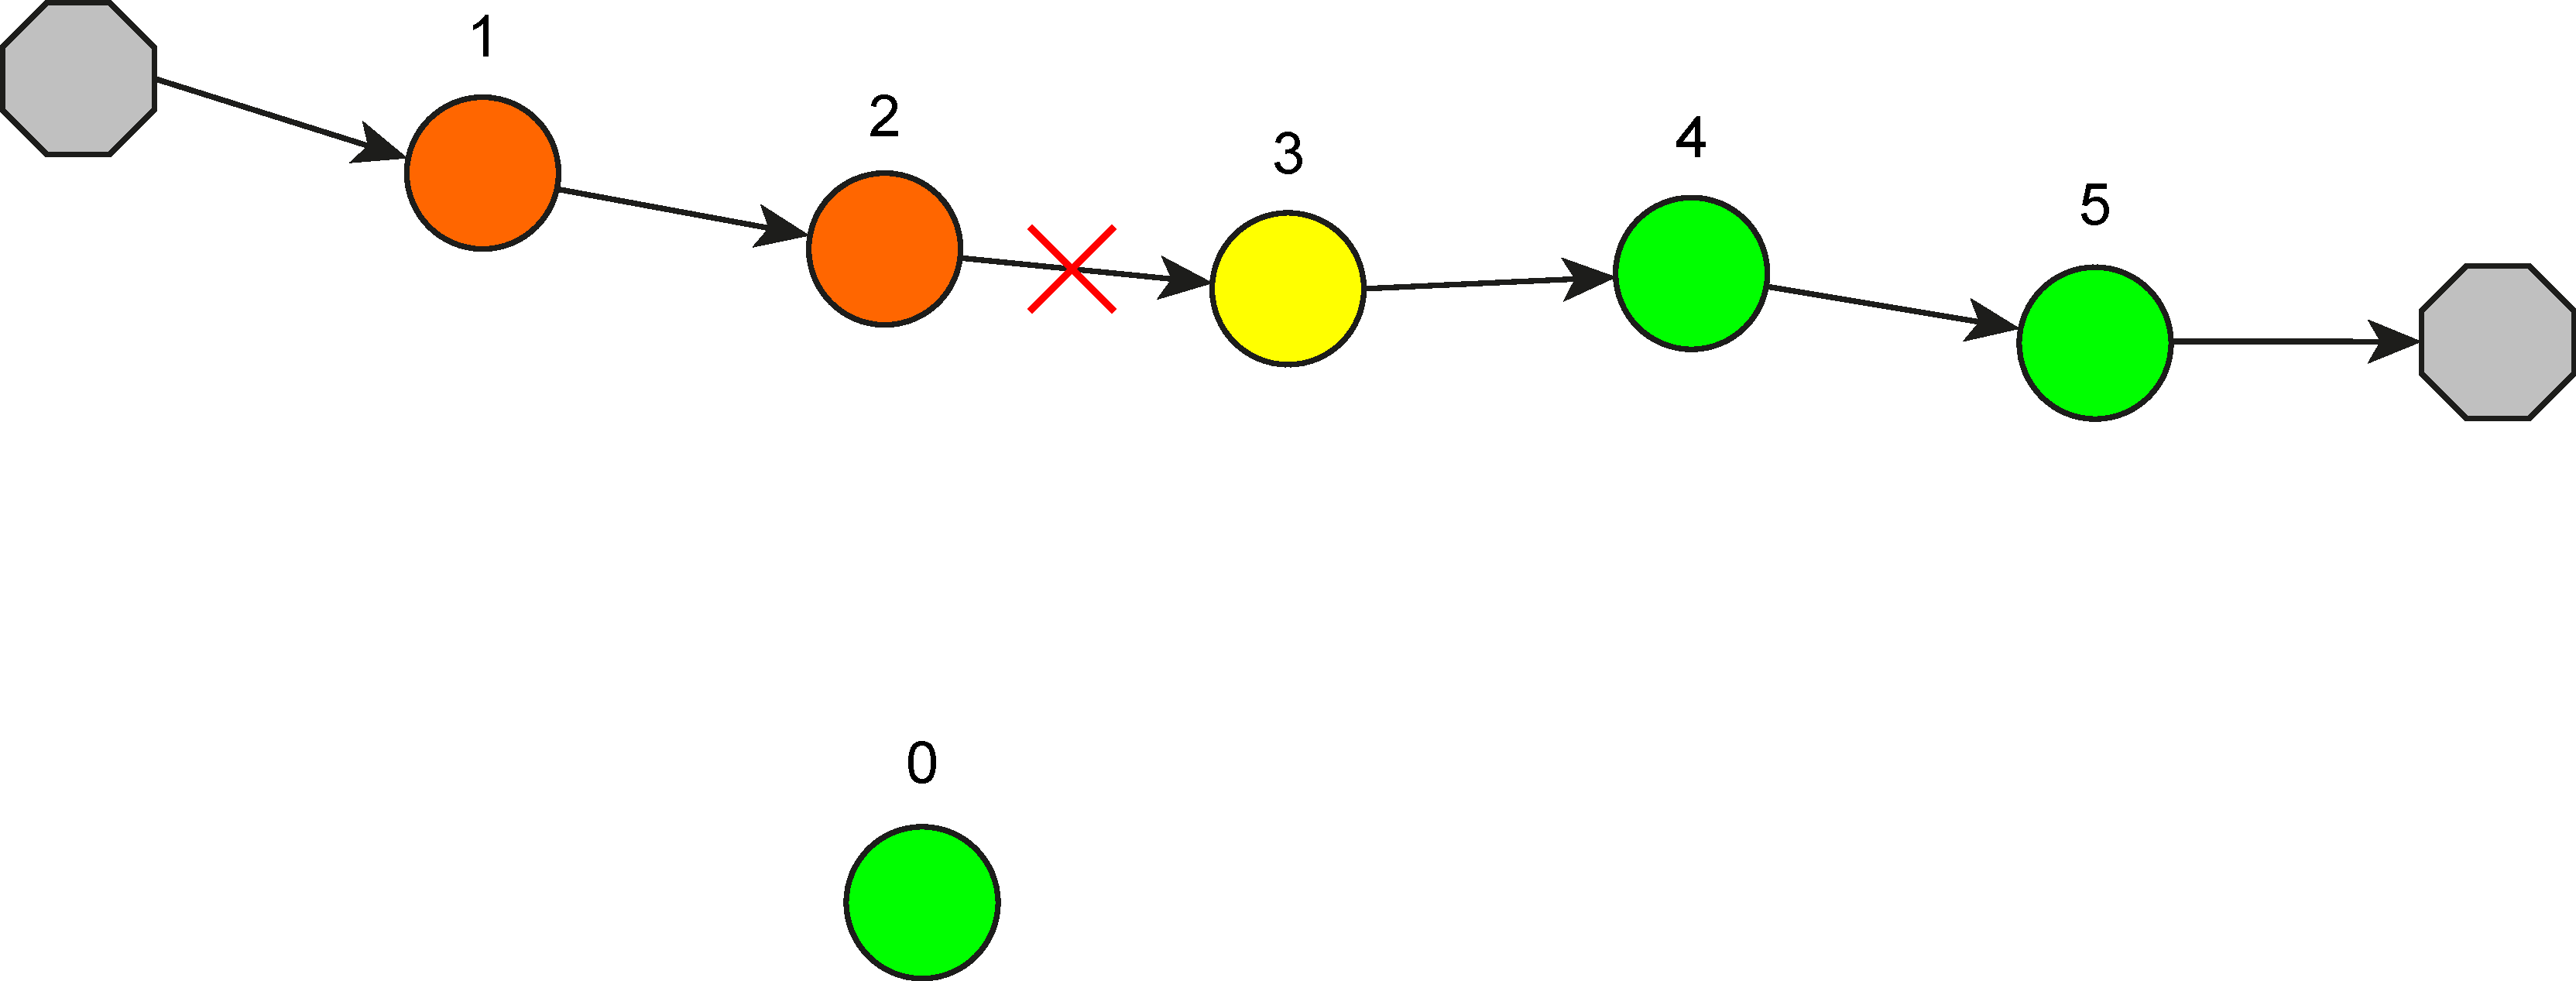
\includegraphics[width=0.45\textwidth,valign=b]{chapters/figures/POMDP_3.pdf}}\smallskip\\
        \subcaptionbox{
            We reconnect substation $3$ (green). State: $s_2 = (2 \mhyphen 3, 3, \{1,2\})$.
            \label{5}}
            {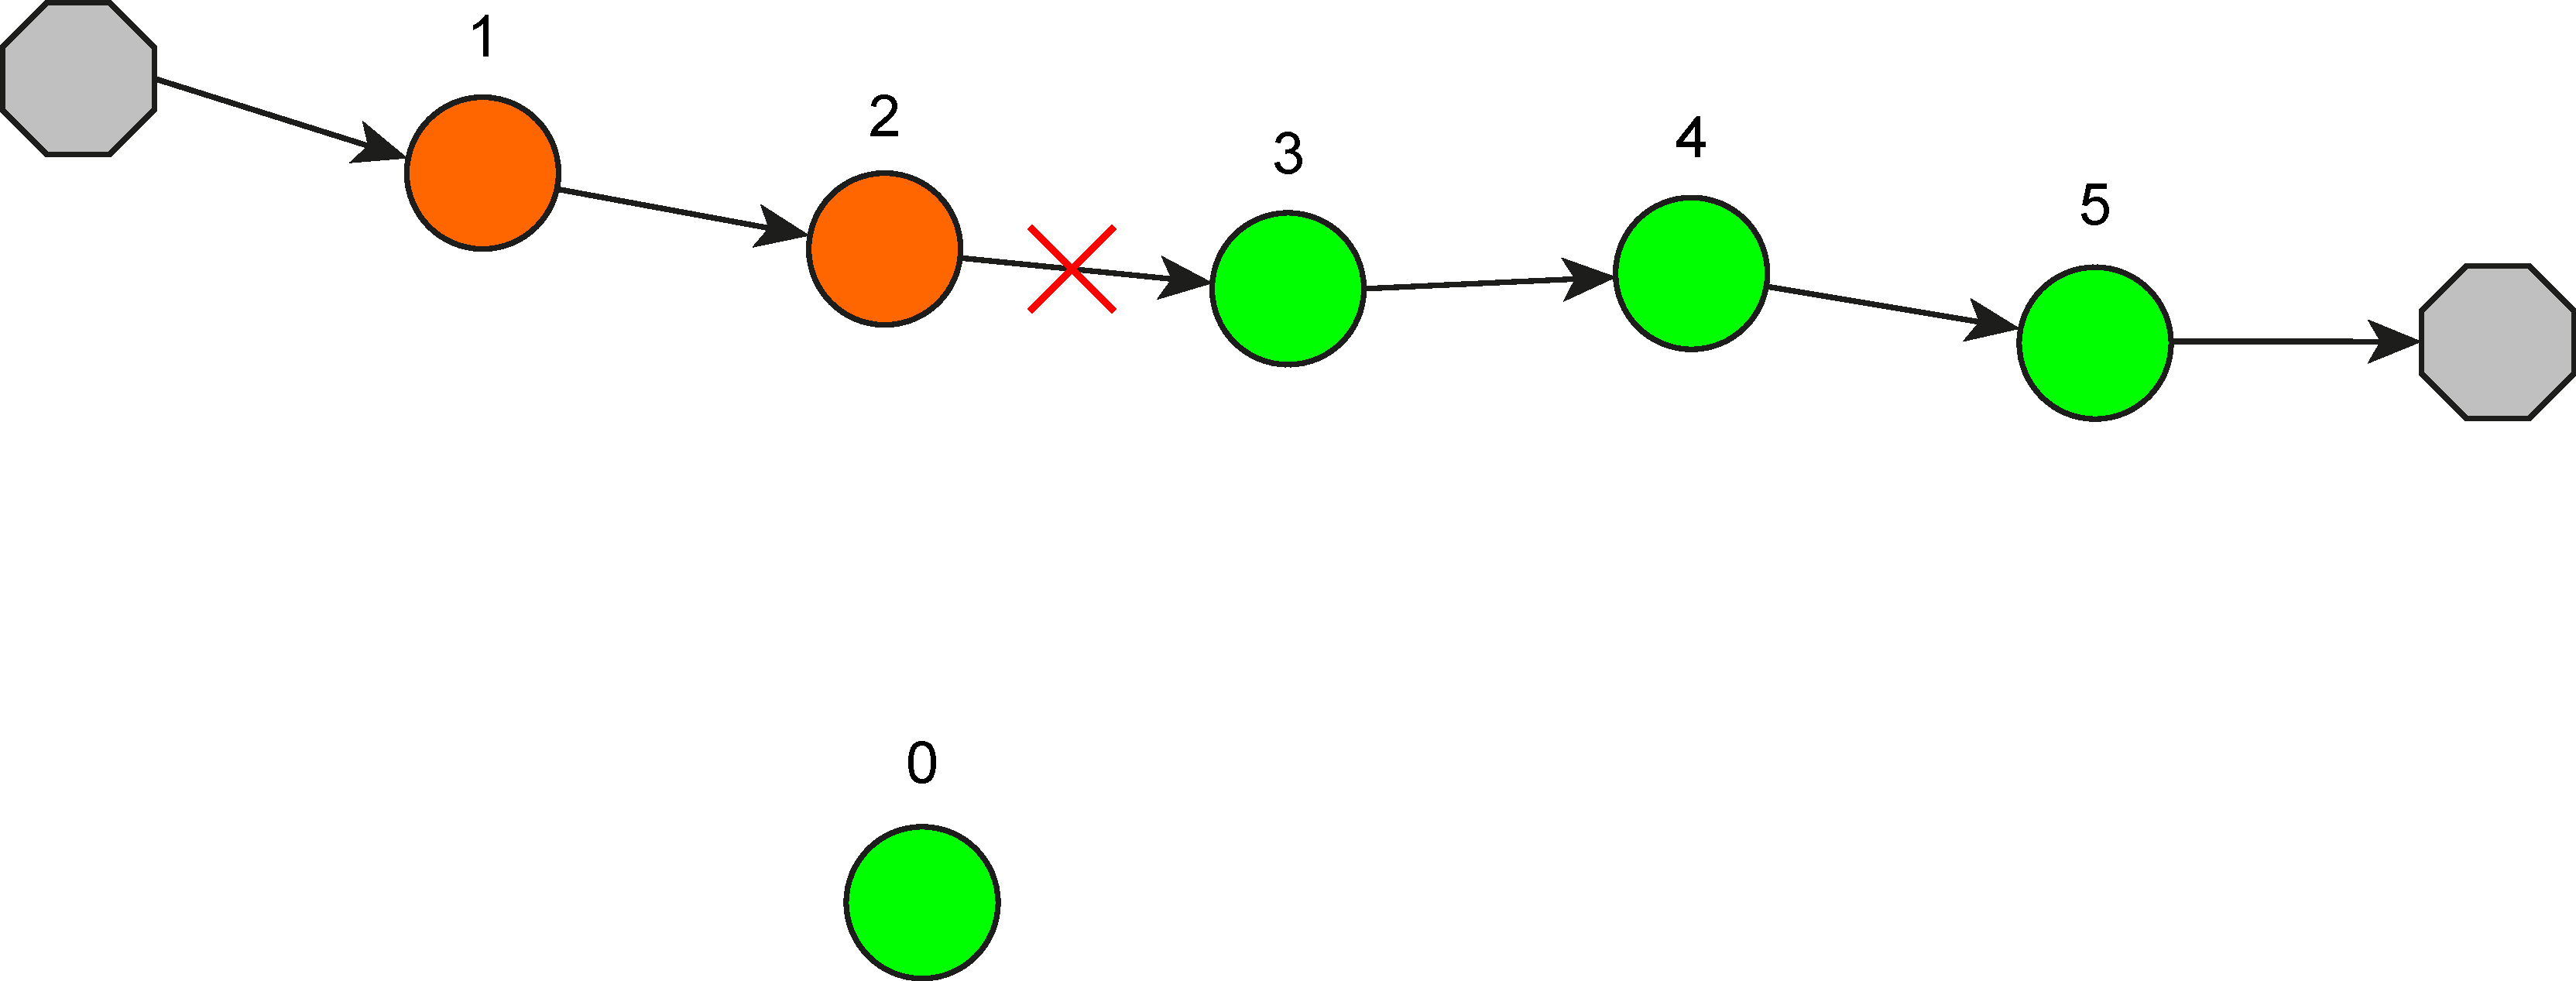
\includegraphics[width=0.45\textwidth,valign=b]{chapters/figures/POMDP_4.pdf}} &
        \subcaptionbox{
            We visit substation $2$ (yellow).\\ Action: $a_2 = 2$.
            \label{6}}
            {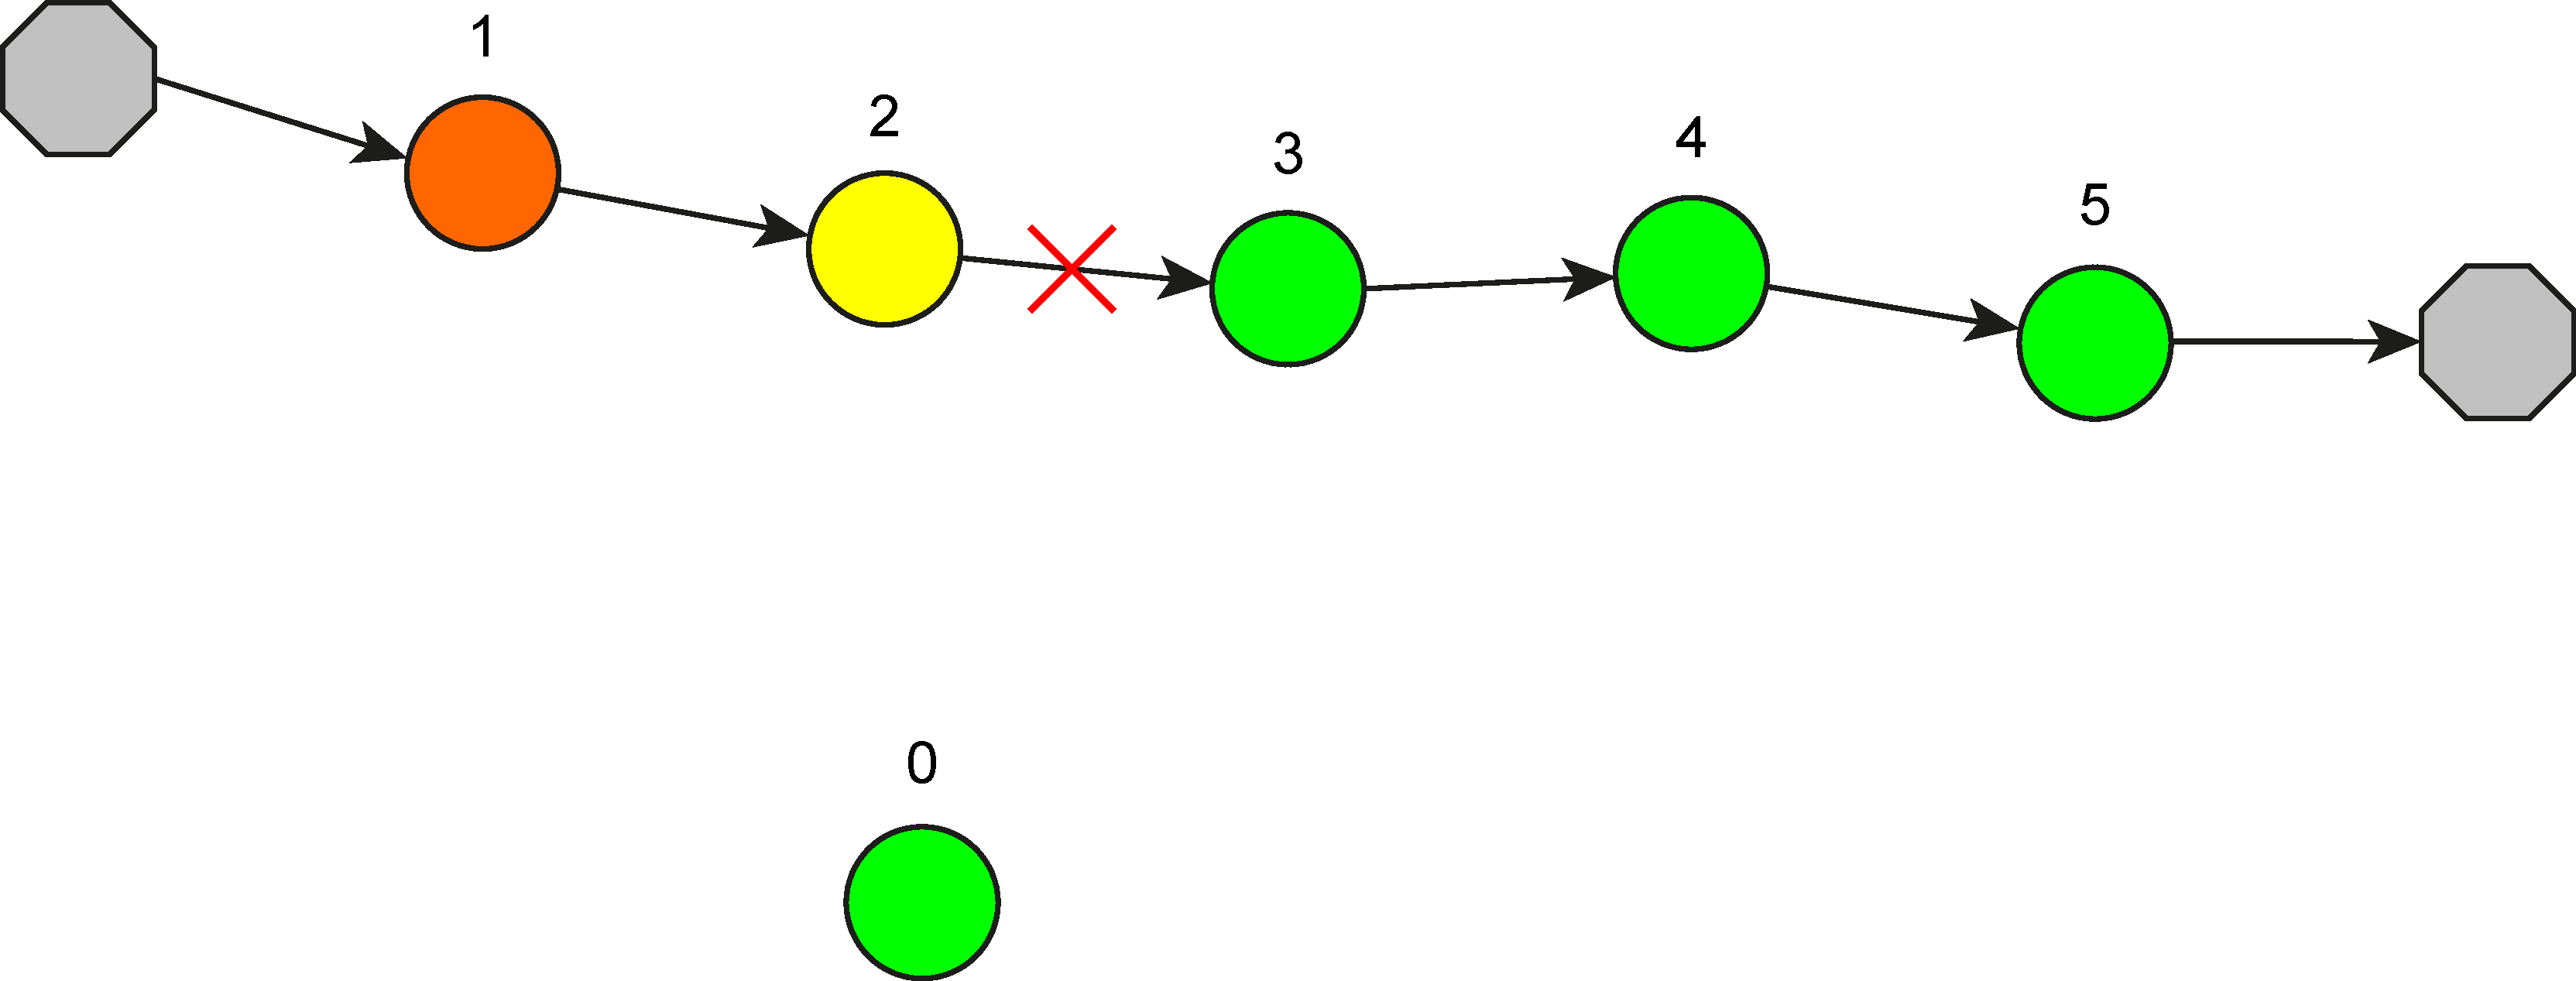
\includegraphics[width=0.45\textwidth]{chapters/figures/POMDP_5.pdf}}\medskip\\
    \end{tabular}
    \subcaptionbox{
        We reconnected substations $1$ and $2$ (green). All the substations are reconnected. Terminal state: $s_3 = (2 \mhyphen 3, 2, \varnothing)$.
        \label{7}}
        {\makebox[0.92\textwidth][c]{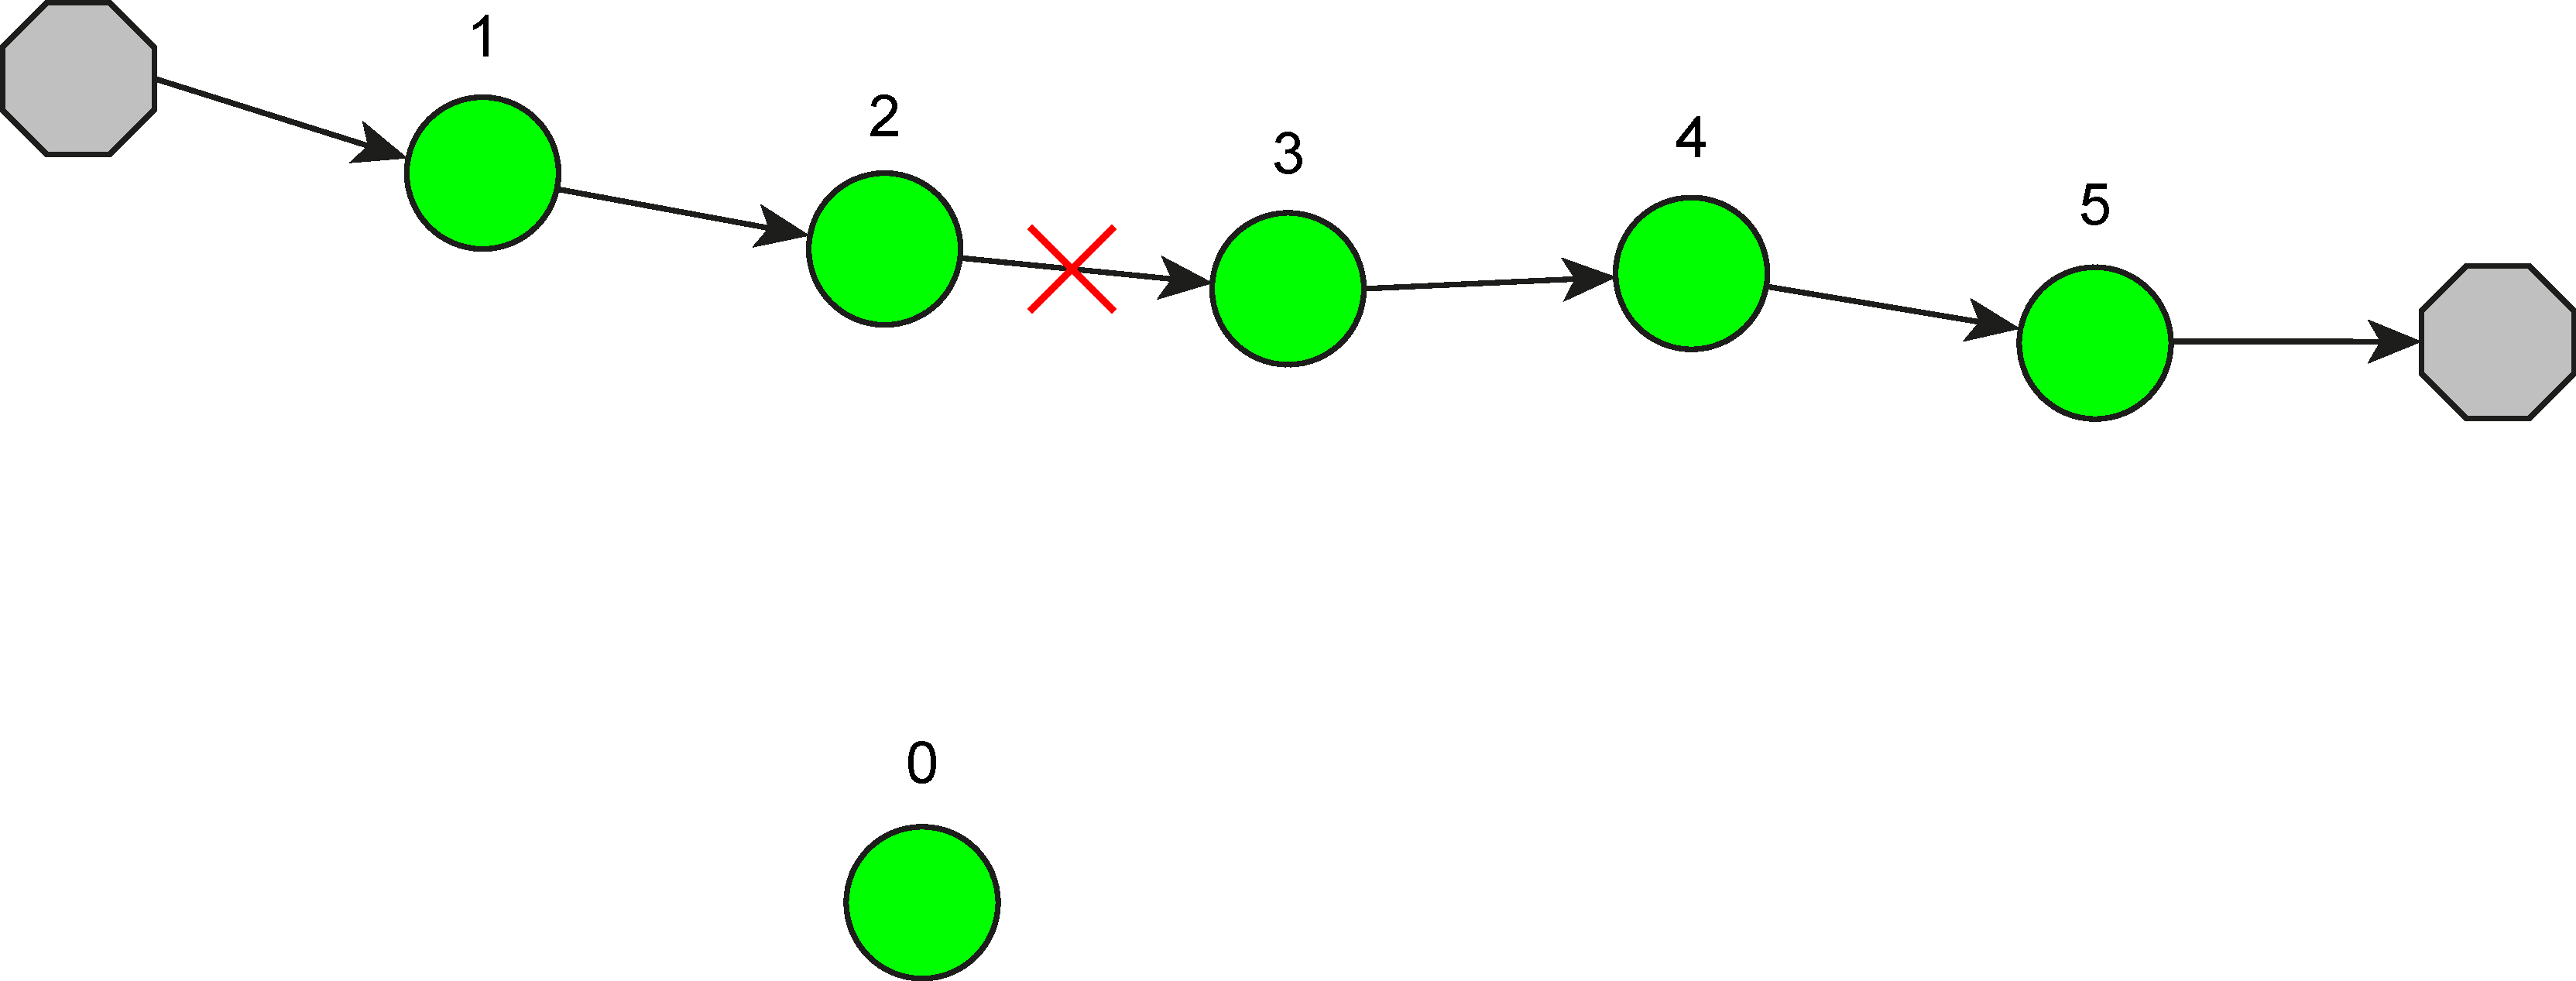
\includegraphics[width=0.45\textwidth]{chapters/figures/POMDP_6.pdf}}}
    \caption{Fictional example of the sequence of actions of the technician, from the occurrence of the fault to its resolution. The fault is in the electrical cable between substations $2$ and $3$, and the gray octagonal substations are the remotely controlled ones, while the round substations are the disconnected ones, except substation $0$, which is the initial position of the technician.}
    \label{fig:sequence-substations}
    \vspace{-17pt} % To remove warning that the image is too long
\end{figure}

The environment is \emph{deterministic}, so given an admissible action $a$, we will surely perform it and end up in the state to which that action leads. We can say that there are no execution errors, and we will always do what we want to do. This means that the next state $s'$ is a function of the previous state $s$ and the action $a$ performed: $s' = \sigma(s,a)$. So, mathematically, we have that the \emph{transition probability}\index{transition probability} is
\begin{equation}
    p(s' \mid s, a) = \mathbb I\big(s' = \sigma(s, a)\big) = \delta_{s', \sigma(s,a)} = \begin{cases} 1 & \text{if } s'=\sigma(s,a) \\ 0 & \text{otherwise} \end{cases} \,,
\end{equation}
where $\mathbb I$ is the characteristic function of a set, and $\delta$ is the Kronecker delta. In our specific case, the transition probability is equal to $1$ only when, starting from state $s = (x_g, v_k, \{v\})$, the new substation $v_{k+1}$ of the next state $s' = (x_g, v_{k+1}, \{v'\})$ is equal to the action $a \in \{v\}$ that we took, so:
\begin{equation}
    p(s' | s,a) = \begin{cases}
        1 & \text{if } v_{k+1} = a \\
        0 & \text{if } v_{k+1} \neq a
    \end{cases} \,.
    \label{eq:transprob}
\end{equation}


\subsection{Policy parametrization}

Given that we are in a situation of partial observability, as we don't know the position of the fault, the \emph{policy}\index{policy} depends only on the observables and not on the state, so it doesn't know where the fault is. Let's define a parameterized policy using a simple \emph{tabular} parameterization, in which we have a parameter $\theta_{o,a}$ for each observable $o$ and action $a$ pair:
\begin{equation}
    \boldsymbol \theta = (\theta_{o,a})_{o \in \mathcal O, a \in \mathcal A} = \begin{pmatrix}
        \theta_{o_1, a_1} & \theta_{o_1, a_2} & \cdots & \theta_{o_1, a_N} \\
        \theta_{o_2, a_1} & \theta_{o_2, a_2} & \cdots & \theta_{o_2, a_N} \\
        \vdots            &                   &        & \vdots            \\
        \theta_{o_{|\mathcal O|}, a_1} & \theta_{o_{|\mathcal O|}, a_2}  & \cdots &  \theta_{o_{|\mathcal O|}, a_N} \\
    \end{pmatrix}
\end{equation}
(where we recall that $N$ is the number of substations initially disconnected, so the number of possible actions: $|\mathcal A| = |\mathcal C| = N$).

Then we use the soft-max, or Boltzmann, distribution of \eqref{eq:pi-boltzmann} to construct the policy:
\begin{equation}
    \pi \Big( a \;\big|\; o(s) = (v_k, \{v\}); \boldsymbol \theta \Big) = \frac{e^{\theta_{o,a} }}{\sum_{b \in \{v\}} e^{\theta_{o,b} }} \,.
    \label{eq:parameterizedpolicy}
\end{equation}

So we have that also the policy is a matrix:
\begin{equation}
    \pi \Big( a \;\big|\; o(s); \boldsymbol \theta \Big) = \begin{pmatrix}
        \pi(a_1 | o_1; \boldsymbol \theta) & \pi(a_2 | o_1; \boldsymbol \theta) & \cdots & \pi(a_N | o_1; \boldsymbol \theta) \\
        \pi(a_1 | o_2; \boldsymbol \theta) & \pi(a_2 | o_2; \boldsymbol \theta) & \cdots & \pi(a_N | o_2; \boldsymbol \theta) \\
        \vdots            &                   &        & \vdots            \\
        \pi(a_1 | o_{|\mathcal O|}; \boldsymbol \theta) & \pi(a_2 | o_{|\mathcal O|}; \boldsymbol \theta)  & \cdots &  \pi(a_N | o_{|\mathcal O|}; \boldsymbol \theta) \\
    \end{pmatrix} \, .
\end{equation}
The policy cannot depend on the position of the failure, otherwise we would automatically have solved the problem: the policy would suggest going in the substation in which the fault is, or in the two substations at the ends of the faulty electrical cable.

Note that what matters in \eqref{eq:parameterizedpolicy} is not the absolute value of the parameters, but only the relative value of a parameter over another one: if we add a constant $c \in \mathbb R$ to all the parameters, there is no effect on the action probabilities, since the constant cancels out:
\begin{equation}
    \frac{e^{\theta_{o,a} + c}}{\sum_{b \in \{v\}} e^{\theta_{o,b} + c}}
    = \frac{e^c\cdot e^{\theta_{o,a} }}{e^c \sum_{b \in \{v\}} e^{\theta_{o,b}}}
    = \frac{e^{\theta_{o,a} }}{\sum_{b \in \{v\}} e^{\theta_{o,b} }}
    = \pi( a \mid o(s); \boldsymbol \theta) \, .
    \label{eq:policy-plus-constant}
\end{equation}
Initially, all parameters are the same and depend neither on the observation nor on the action (e.g., $\boldsymbol \theta = \mathbf 0$, thus $\theta_{o,a} = 0$ for all $o \in \mathcal O, a \in \mathcal A$), so that all actions have an equal probability of being selected. This is called the \emph{random policy}, and in our case is
\begin{equation}
    \pi \left( a \;\big|\; o(s); \boldsymbol \theta \right) = \frac{e^{\theta}}{\sum_{b \in \{v\}} e^{\theta}} = \frac{e^{\theta}}{e^\theta \sum_{b \in \{v\}} 1 } = \frac1{ |\{v\}| } \, ,
    \label{eq:rndpolicy}
\end{equation}
which means that we randomly choose a substation to visit, since they all have the same uniform probability. Actually, this is true for every choice of $\boldsymbol \theta$ which doesn't depend on the observation-action pair, so also any other constant $c \in \mathbb R$ would do (as we can see from \eqref{eq:policy-plus-constant}), but in practice, to construct a uniform policy, one usually takes $\boldsymbol \theta = \mathbf 0$.

One of the advantages of using the soft-max distribution to parameterize policies is that, in the learning phase, we are able to choose a random action without introducing and manually tuning a $\varepsilon$ term, which we would otherwise need to perform some exploration alongside the exploitation. Instead, the stochasticity is intrinsic, since we don't perform a deterministic maximization over the actions, but we choose it according to its probability. In particular, if the optimal policy is stochastic, an $\text{argmax}$ would never be able to approximate it, not even with a $\varepsilon$ parameter, while the soft-max can do it by construction. On the contrary, if an action is deterministic, the soft-max can approach it as close as possible; in fact, the approximate policy can approach a deterministic policy without any problem. 

If we search in this space of parametrized policies, this will give us a policy that doesn't depend on time, but only on the parameters, which we want to optimize. This means that, by construction, we have a \emph{stationary policy}. The reason for this choice is that, in our problem, the time is not encoded like a problem of dynamic programming, in which we have a well-defined sequence of time steps. The structure of the states is already a measure of time, as the number of moves already done: the sequence of substations we already visited. So what is important is not to establish a policy at different time steps, but to create a policy with respect to the states (in our case with respect to the observables).


\subsection{Value function and performance measure}

In our problem, the equation for the \emph{action value function}\index{action value function} $Q_\pi(s,a)$ in \eqref{eq:Q-recursive}, given that the state is $s = ( \, x_g, o = (v_k, \{v\}) \, )$, the action is $a \in \{v\}$ and the next state is $s' = ( \, x_g, o' = (v_{k+1}=a, \{v'\}) \, ) = \sigma(s,a)$ (since the system is deterministic), becomes, thanks to \eqref{eq:expected-reward} and \eqref{eq:transprob},
\begin{equation}
    \begin{aligned}
        Q_\pi(s,a)
        &= \sum_{s'} p(s' \mid s, a) \left[ r(s,a,s') + \sum_{a'} \pi(a'|o(s'); \boldsymbol \theta)  Q_\pi (s', a') \right] \\
        &= \left(d_{v_k, a} \cdot n_{k} + \sum_{a' \in \{v'\}} \pi \Big( a' \big| o \big( \sigma(s,a) \big); \boldsymbol \theta \Big) \, Q \big( \sigma(s,a), a' \big) \right) \, .
    \end{aligned}
    \label{eq:myQ}
\end{equation}

Now, let us find the formula for $\rho_0(s')$, the probability of starting in state $s'$. Since we have no prior information on where the fault might be, $\rho_0$ doesn't depend on it, so it will be uniform in $x_g$. The fault can happen either in one of the substations, which are $|\mathcal C| = N$, or on one of the electrical cables, which are $N+1$, so the number of possible $x_g$ is $N + (N+1) = 2N+1$. In an initial state, the current position of the technician $v_k$ must be the dummy substation $0$, which represents the position of the technician when the fault occurs, and the set of the disconnected substations must be equal to the set of all the substations $\mathcal C$. So $\rho_0$ must be $1$ when the current substation is $0$ and the set of the disconnected substations is equal to $\mathcal C$, and must be $0$ for every other situation. In other words, we have that
\begin{equation}
    \begin{aligned}
        \rho_0 \Big(s = ( \, x_g, o =(v_k, \{v\}) \,) \Big)
        &= \text{Pr}(x_g) \mathbb I (o = o_0 = (0, \mathcal C)) \\
        &= \frac1{2N+1} \mathbb I \big( v_k = 0, \{v\} = \mathcal C \big) \\
        &= \frac1{2N+1} \delta_{o(s), o_0} \, ,
    \end{aligned}
    \label{eq:myrho}
\end{equation}
where $o_0$ is the initial observation, and in the last equivalence we used the Kronecker delta $\delta$. Actually, according to the technicians of the \acrshort{aaa} company, the majority of the faults happens on the electrical cables, usually when they are no longer perfectly isolated. We will try to take advantage of this information at a later moment, but for now we will suppose that every component has the same probability of being damaged.

Moreover, the formula \eqref{eq:eta} for the function $\eta_\pi(s')$ in our case becomes, thanks to \eqref{eq:transprob} and \eqref{eq:myrho},
\begin{equation}
    \begin{aligned}
        \eta_\pi\Big(s' = (\, x_g, o'=(v_{k+1}, \{v'\}) \,) \Big)
        &:= \rho_0(s') + \sum_s \eta_\pi(s) \sum_a \pi(a | o(s); \boldsymbol \theta) p(s' | s, a) \\
        &= \frac1{2N+1} \delta_{o', o_0} + \sum_{s \in \mathrm{pa}(s')} \eta_\pi(s) \pi(v_{k+1} | o(s); \boldsymbol \theta) \, ,
    \end{aligned}
    \label{eq:myeta}
\end{equation}
where $\mathrm{pa}(s')$ indicates the parents of the node $s'$ in the states' dependency graph, which represents all the possible sequences of states.

Finally, let us define the \emph{performance measure}\index{performance measure} $J_\pi(\boldsymbol \theta)$ as the sum of all the costs we incur, added up over time until the process is concluded. Actually, the time steps of the process are merely formal steps, since we don't keep track of the time passed, but we simply move from one substation to another. Thus, the actual physical time is in the costs, as the cost of going from one substation to another, which we measure using the time it takes to drive between them. Given the definition of $J_\pi(\boldsymbol \theta)$ as in \eqref{eq:J}, in our case we have that
\begin{equation}
    \begin{aligned}
        J_\pi(\boldsymbol \theta) 
        &= \sum_s \rho_0(s) \sum_a \pi_{\boldsymbol \theta} (a|o(s); \boldsymbol \theta) \, Q_{\pi_{\boldsymbol \theta}}(s,a) \\
        &= \sum_{s} \frac{1}{2N+1} \delta_{o(s), o_0} \sum_a \pi_{\boldsymbol \theta} (a|o(s); \boldsymbol \theta) \, Q_{\pi_{\boldsymbol \theta}}(s,a) \\
        &=  \sum_{x_g} \frac{1}{2N+1} \sum_a \pi_{\boldsymbol \theta} (a|o_0; \boldsymbol \theta) \, Q_{\pi_{\boldsymbol \theta}} \big( (x_g, o_0),a \big) \, ,
    \end{aligned}
    \label{eq:myJ}
\end{equation}
where in the second equivalence we used equation \eqref{eq:myrho}, and the last equivalence derives from the fact that the sum $\sum_s \delta_{o(s), o_0}$ is equivalent to a summation over every possible position of the fault for the initial observation $o_0$. In particular, $(x_g, o_0)$ represents every possible initial state for different positions of the fault.


\subsection{Policy gradient method}

Since we know every aspect of the problem, and we have a model of the environment, we can solve it via a \emph{model-based method}\index{model-based method}. Due to the partial observability, though, we cannot use \emph{dynamic programming} methods like the ones in \cite{BellmanDP}, because we would need a policy that depends on the entire state, thus also on the hidden variable $x_g$. However, if we know where the fault is, the optimal solution is straightforward: if it is on an electrical cable, we need to visit the two substations at the ends of it (we might have to choose the right order); if it is in a substation, we visit it directly. Thus, we need an algorithm that can work in a \acrshort{pomdp}.

We will use one of the \emph{policy gradient methods}\index{policy gradient method} of \autoref{sec:pgm} in the \acrshort{pomdp}, since they can naturally handle partial observability. In particular, we will perform a \emph{gradient descent}\index{gradient descent} --- since we want to \textit{minimize} our \textit{cost} $J_\pi(\boldsymbol \theta)$ --- on the parameters $\boldsymbol \theta$ of the policy $\pi_{\boldsymbol \theta}$, where we said that the latter depends only on the observations, and so will do the gradient.

The formula of the gradient in \eqref{eq:gradJ} in our case becomes
\begin{equation}
    \nabla_{\boldsymbol \theta} J_\pi (\boldsymbol \theta) = \sum_{s \in \mathcal S} \eta_{\pi_{\boldsymbol \theta}}(s) \sum_{a \in \mathcal A(s)} Q_{\pi_{\boldsymbol \theta}}(s,a) \nabla_{\boldsymbol \theta} \pi(a|o(s); \boldsymbol \theta) \, .
    \label{eq:mygradJ_oneline}
\end{equation}

So, given that $\boldsymbol \theta$ is a matrix $\boldsymbol \theta = (\theta_{o,a})_{o \in \mathcal O, a \in \mathcal A}$, we have that also the gradient is a matrix:
\begin{equation}
    \nabla_{\boldsymbol \theta} J_\pi (\boldsymbol \theta) = \begin{pmatrix}
        \frac{\partial}{\partial \theta_{o_1, a_1}} J & \cdots & \frac{\partial}{\partial \theta_{o_1, a_N}} J \\
        \frac{\partial}{\partial \theta_{o_2, a_1}} J &  \cdots & \frac{\partial}{\partial \theta_{o_2, a_N}} J \\
        \vdots \\
        \frac{\partial}{\partial \theta_{o_{|\mathcal O|}, a_1}} J & \cdots & \frac{\partial}{\partial \theta_{o_{|\mathcal O|}, a_N}} J
    \end{pmatrix} \, ,
\end{equation}
where $N = |\mathcal A| = |\mathcal C|$ is the number of initially disconnected substations.

First of all, let us compute the gradient of the policy $\pi$. Given the equation of the policy in $\eqref{eq:parameterizedpolicy}$, we have that its derivative is
\begin{equation}
    \begin{aligned}
        \frac{\partial}{\partial \theta_{o',a'}} \pi \Big( a \;\big|\; o=(v_k, \{v\}); \boldsymbol \theta \Big)
        &= \frac{\partial}{\partial \theta_{o',a'}} \left( \frac{e^{\theta_{o,a} }}{\sum_{b \in \{v\}} e^{\theta_{o,b} }} \right) \\
        &= \delta_{o',o} \cdot \frac{\delta_{a',a} \cdot e^{\theta_{o,a} } \cdot \sum_{b \in \{v\}} e^{\theta_{o,b} } -  e^{\theta_{o,a} } \cdot e^{\theta_{o, a'} }}{(\sum_{b \in \{v\}} e^{\theta_{o,b}})^2} \\
        &= \delta_{o',o} \cdot \left( \frac{\delta_{a',a} \cdot e^{\theta_{o,a} } \cdot \sum_{b \in \{v\}} e^{\theta_{o,b} }}{(\sum_{b \in \{v\}} e^{\theta_{o,b} })^2} - \frac{e^{\theta_{o,a} }}{\sum_{b \in \{v\}} e^{\theta_{o,b} }}\cdot\frac{e^{\theta_{o,a'} }}{\sum_{b \in \{v\}} e^{\theta_{o,b} }} \right) \\
        &= \delta_{o',o} \cdot \left( \delta_{a',a} \pi(a|o; \boldsymbol \theta) - \pi(a|o; \boldsymbol \theta) \pi(a'|o; \boldsymbol \theta) \right) \\
        &= \delta_{o',o} \left( \delta_{a',a} - \pi(a'|o; \boldsymbol \theta) \right) \, \pi(a|o; \boldsymbol \theta)  \, ,
    \end{aligned}
    \label{eq:gradpi}
\end{equation}
since if $o \neq o'$ we have that $\theta_{o',a'}$ and $\theta_{o,a}$ are ultimately different parameters. In particular, for the random policy (so when $\boldsymbol \theta = \mathbf 0$) we have that
\begin{equation}
    \left. \frac{\partial}{\partial \theta_{o',a'}} \pi \Big( a \;\big|\; o=(v_k, \{v\}); \boldsymbol \theta \Big) \right|_{\boldsymbol \theta = \mathbf 0}
    = \delta_{o',o} \left(\frac1{|\{v\}|} \delta_{a',a} - \frac1{|\{v\}|^2} \right)
    \label{eq:deriv-pi}
\end{equation}
The gradient of the policy is, in general, a tensor with dimensions $|\mathcal O| \times |\mathcal A| \times |\mathcal O| \times |\mathcal A|$. For a fixed observation $o$ and for a fixed action $a$, however, it reduces to the following matrix:
\begin{equation}
    \nabla_{\boldsymbol \theta} \pi(a|o; \boldsymbol \theta) = \begin{pmatrix}
        \frac{\partial}{\partial \theta_{o_1,a_1}} \pi ( a | o; \boldsymbol \theta )
            %& \frac{\partial}{\partial \theta_{o_1,a_2}} \pi ( a | o; \boldsymbol \theta )
            & \cdots & \frac{\partial}{\partial \theta_{o_1,a_N}} \pi ( a | o; \boldsymbol \theta ) \\
        \vdots & &
        %&
        \vdots \\
        \frac{\partial}{\partial \theta_{o_{|\mathcal O|},a_1}} \pi ( a | o; \boldsymbol \theta ) 
            %& \frac{\partial}{\partial \theta_{o_{|\mathcal O|},a_2}} \pi ( a | o; \boldsymbol \theta )
            & \cdots & \frac{\partial}{\partial \theta_{o_{|\mathcal O|},a_N}} \pi ( a | o; \boldsymbol \theta ) \\
    \end{pmatrix}
\end{equation}

Given this, we have that
\begin{equation}
    \begin{aligned}
        \nabla_{\theta_{o',a'}} J_\pi (\boldsymbol \theta)
        &= \sum_{s \in \mathcal S} \eta_\pi(s) \sum_{a \in \mathcal A(s)} Q_\pi(s,a) \nabla_{\theta_{o',a'}} \pi(a|o(s)) \\
        &= \sum_s \eta_\pi(s) \sum_a Q_\pi(s,a) \delta_{o',o(s)} \Big( \big( \delta_{a',a} - \pi(a'|o(s)) \big) \, \pi(a|o(s)) \Big) \\
        &= \sum_{x_g} \eta_\pi \big((x_g, o') \big) \sum_a Q_\pi \big((x_g, o'),a \big) \big( \delta_{a,a'} - \pi(a'|o') \big) \, \pi(a|o') \, ,
    \end{aligned}
    \label{eq:mygradJ}
\end{equation}
where, as we did in equation \eqref{eq:myJ}, the sum $\sum_s \delta_{o', o(s)}$ is equivalent to a summation over every possible position of the fault for the specific observation $o'$ on which we are deriving. In particular, $(x_g, o')$ is the state with a fault at some position $x_g$ and with observation $o'$.

The idea of the algorithm is the following. We start from a certain policy, for example, the random policy of equation \eqref{eq:rndpolicy}, in which we choose randomly the substation to be visited. Then we compute the gradient for every parameter using \eqref{eq:mygradJ}. As we saw in \eqref{eq:deriv-pi}, the gradients of the policy are simple computations (since we decided the parametrization of the policy, we were able to derive their formulas), while the computations for the objects $Q_\pi$ and $\eta_\pi$ have to be done indirectly: we have to solve the linear equations \eqref{eq:myQ} and \eqref{eq:myeta} for the current policy, which can be more or less computationally heavy, also depending on the method chosen.
%Given the form of our transition probabilities $p(s' | s, a)$, we have that the equations of $Q_\pi$ do not depend on $s'$, but only on the current state $s$ and the action $a$. So, fixed the first state $s$, we have to solve two linear equations only on the actions (we can see the $Q(s,a)$ matrix as a series of vectors).

Having done these steps, we have the value of the gradient for every parameter. Then we take a step in the parameters space, and we descend the gradient. We stop when the value of $J_\pi (\boldsymbol \theta)$ doesn't change much in percentage.

In general, there is no guarantee that this is a convex problem in the parameters $\boldsymbol \theta$, on the contrary, we could have several minima. Therefore, we should perform different gradient descents starting with some policies different from the one which has $\boldsymbol \theta = \mathbf 0$, to see if we can reach a different minimum, or if we always reach the same one. These are called random restarts. Of course, this doesn't guarantee finding the global minimum, but it is the best we can do to at least check that we are not stuck in a local minimum. For the random restarts, we chose the parameters $\boldsymbol \theta$ from a standard normal distribution $\mathcal N(0,1)$, in order to have both positive values and negative ones to start from.

If we have the intuition that there is a deterministic sequence of actions to be performed, we have that their parameters $\theta_{\cdot,a}$ tend to infinity. This is because the deterministic policies correspond to a matrix of one-hot vectors --- in which we have $1$ for only one action and $0$ for all the other ones, which in the soft-max policy happens when the parameter associated with this action becomes much bigger than the others. If it is so, the gradient descent never stops and there could be problems of overflowing on the values of the policy, since the parameters $\boldsymbol \theta$ can become very large, and the exponentials of the soft-max would explode. A smart thing to do when this happens is to rewrite the parametrization in the following way (the observation $o$ is fixed):
\begin{equation}
    \pi(a | o) = \frac{e^{\theta_{o,a}}}{\sum_b e^{\theta_{o,b}}} = \frac{e^{-(\max_{a'} \theta_{o,a'} - \theta_{o,a})}}{\sum_b e^{-(\max_{a'} \theta_{o,a'} - \theta_{o,b})}} \, .
    \label{eq:pi-clipped}
\end{equation}
The benefit of writing the policy in this way is that, since the exponents of the two exponentials are negative (the parts in the parenthesis, $\max_{a'} \theta_{o,a'} - \theta_{o,\cdot}$, are always positive), it never explodes. In fact, negatives with large exponents ``saturate'' to zero rather than infinity, so we have a better chance of avoiding NaNs. This is a simple numerical trick that allows improving the stability of the algorithm. %([link](https://eli.thegreenplace.net/2016/the-softmax-function-and-its-derivative/))


\subsubsection{Natural policy gradient}

Following what we said in \autoref{sec:npg}, and given that the derivative of our policy is \eqref{eq:gradpi}, we have that

\begin{equation}
    \widetilde \nabla_{\theta_{o',a'}} \pi(a|o(s)) = I_{(\mathcal O, \mathcal A) \times (\mathcal O, \mathcal A)} = \delta_{o', o(s)} \delta_{a',a} \, .
\end{equation}

Then the equation of the natural gradient of the performance measure $J(\boldsymbol \theta)$ of \eqref{eq:natgradJ}, which was
\begin{equation*}
    \widetilde \nabla_{\boldsymbol \theta} J(\boldsymbol \theta) = F^{-1}(\boldsymbol \theta) \nabla_{\boldsymbol \theta} J(\boldsymbol \theta) \, ,
\end{equation*}
in our case becomes, thanks to the equation of the natural gradient of $\pi$ used in equation \eqref{eq:mygradJ_oneline},
\begin{equation}
    \begin{aligned}
        \widetilde \nabla_{\theta_{o',a'}} J_\pi (\boldsymbol \theta)
        &= \sum_{s \in \mathcal S} \eta_\pi(s) \sum_{a \in \mathcal A(s)} Q_\pi(s,a) \widetilde \nabla_{\theta_{o',a'}} \pi(a|o(s)) \\
        &= \sum_s \eta_\pi(s) \sum_a Q_\pi(s,a) \delta_{o', o(s)} \delta_{a',a} \\
        &= \sum_{x_g} \eta_\pi \big((x_g, o') \big) Q_\pi \big((x_g, o'), a' \big)\, .
    \end{aligned}
    \label{eq:mynatgradJ}
\end{equation}

This is a very nice result, in that we have a very simple equation for the gradient of the performance measure $J(\boldsymbol \theta)$, which is also guaranteed to converge faster to a minimum, although not a global one.


\section{Implementation of the model}

First of all, we generated all the states of the system using \emph{backtracking}\index{backtracking}, a technique used to systematically generate all the admissible solutions of a problem (usually of combinatorial nature) \cite{Montresor2014}. It proceeds by incrementally building candidate solutions using recursion, checking at each step if a complete and valid solution is reached, and backtracking to explore other ones. In our case, the function starts from a complete initial state, so, besides the current position of the technician and the set of disconnected substations, it also requires the position of the fault, and it determines all the possible actions that can be taken from that state. Then it computes all the subsequent states, determining each time which substations can be reconnected by doing one of the possible actions, and it continues until it has reconnected all the substations. We can reconstruct all the possible states of the system by looping over all the possible positions of the fault, so on all the possible initial states. While constructing the states, the function also creates the states' dependency graph, in which, given a state, we can find all the possible states in which we can end up doing an admissible action. This is actually a forest of trees: each graph is a tree because we can never return to a previous state, and it is a forest since the states are grouped by the position of the fault: if we start in a given initial state we can never end up in a state with a different position of the fault.

From the list of states, we create the list of observables, and we associate each state to its uniquely defined observation using a dictionary.

After having done that, we proceed to construct the matrix of parameters $\boldsymbol \theta$, initialized to zero, and the matrix of the policy $\pi_{\boldsymbol \theta}$, with the same dimensions of the previous one, using the soft-max parametrization.

Then we proceed with the computation of the matrix of $Q_\pi$. We construct the matrix $R = (R[s,a])_{s \in \mathcal S, a \in \mathcal A}$, which stores the immediate cost of being in state $s$ and doing action $a$, which thanks to \eqref{eq:expected-reward} is:
\begin{equation}
    R[s,a] = r(s,a,s') = d_{v_k, a} \cdot \sum_{v \in \{v\}} u_v \, ,
\end{equation}
if action $a$ is possible in state $s$, otherwise it is zero. Then we use it to initialize the matrix which will store the values of $Q_\pi$. Recall that in the equation \eqref{eq:myQ} for $Q_\pi$, we use the values of $Q_\pi$ of the next states $s'$ to compute the value of $Q_\pi$ for the current state $s$. Thus, we need to use the states' dependency graph from the leaves to the roots to compute the matrix of $Q_\pi$ bottom-up. We perform a personalized \emph{breadth-first-search}\index{breadth-first-search}, or \acrshort{bfs}, on the states' dependency graph, in order to be able to add each next-state contribution to the value of $Q_\pi$ for the current state. A breadth-first-search is an algorithm for exploring a graph, which visits every node and every edge of the latter. In a breadth-first-search, the nodes are visited in order of increasing distance from the source of the visit, where the distance among the source and a generic node is the minimum number of edges in a path among them \cite{Montresor2014}. In our modified \acrshort{bfs}, instead, we start from the terminal states in the leaves, and then we visit all the edges of the graph in a breadth-first-search order, with every edge traversed in the reverse direction in order to arrive at the initial state in the root. In particular, the major modification is that we visit all the out-edges of a node before visiting that node itself, in order to accumulate its $Q_\pi$ value --- by adding all the terms deriving from its children --- before using it to compute the $Q_\pi$ value of another node.

One might wonder why, being \eqref{eq:myQ} a linear system, we didn't use any of the already existing algorithms to solve it. This is because we don't have the matrix of the linear system explicitly, and we don't have an immediate way to create it, but it is required for algorithms like the Gauss elimination method (a direct method) or the Jacobi or Gauss-Seidel methods (iterative ones). So to compute it, we would need to first traverse the graph like we explained, writing the coefficients of the equations' terms of the linear system in $A$. Then we would still have to solve the linear system, for example with one of the previous methods. However, instead of doing these two passages, we can directly solve the system traversing the graph. This applies to the computation of $\eta_\pi$, as well.

After this, we proceed by computing the vector of $\eta_\pi$. In equation \eqref{eq:myeta} we have that, in order to compute the value of $\eta_\pi$ for a state $s'$, we use the values of $\eta_\pi$ of all its preceding states $s$. Thus, we will use the states' dependency graph from the roots to the leaves to compute the $\eta_\pi$ matrix top-down. As we did for the matrix of $Q_\pi$, we perform a modified \acrshort{bfs} on the states' dependency graph, which visits all the edges. Our \acrshort{bfs} visits a node only after all its in-edges have been visited; this ensures that we have accumulated the node's $\eta_\pi$ value, by having added all the terms deriving from its parents, before using it to compute the $\eta_\pi$ value of another node.

We could not have used a depth-first search, or \acrshort{dfs}, to compute $Q_\pi$ and $\eta_\pi$. In a \acrshort{dfs}, contrary to a \acrshort{bfs}, after visiting a node the search proceeds as far as possible from it along a path, until it reaches a node whose adjacent nodes have all already been visited. Then the search goes back along the last edge and continues moving along another path not yet visited \cite{Montresor2014}. Thus, using a \acrshort{dfs}, it would be impossible to visit all the in-edges (or the out-edges in the reverse order) of a node before visiting the node itself.

Having the matrix of the policy $\pi_{\boldsymbol \theta}$ and the matrix of $Q_\pi$, we can compute the performance measure $J_\pi (\boldsymbol \theta)$ using the last equivalence of \eqref{eq:myJ}. Instead, for the computation of the gradient of $J_\pi (\boldsymbol \theta)$, $\nabla_{\boldsymbol \theta} J_\pi (\boldsymbol \theta)$, we also use the matrix $\eta_\pi$, following equation \eqref{eq:mygradJ}. Since the convergence with the ordinary gradient was quite slow, we also implemented the natural gradient $\widetilde \nabla_{\boldsymbol \theta} J_\pi (\boldsymbol \theta)$, following equation \eqref{eq:mynatgradJ}. Given the higher values of $\boldsymbol \theta$ that the natural gradient can achieve, it is mandatory to implement the clipped version of the policy \eqref{eq:pi-clipped}.

How to choose the learning parameter $\alpha$\index{learning rate} appropriately? We want the difference $\boldsymbol \theta_{k+1} - \boldsymbol \theta_k$ in \eqref{eq:grad-descent} to be small; in particular, we want $\boldsymbol \theta_{k+1} - \boldsymbol \theta_k \ll 1$, therefore, we must have $\alpha \, |\nabla_{\boldsymbol \theta} J_\pi (\boldsymbol \theta)| \ll 1$. Given that we typically have $Q_\pi \sim 10^7$ and $\eta_\pi \sim 10^{-2}$ in the expression of $\nabla_{\boldsymbol \theta} J_\pi (\boldsymbol \theta)$, we choose $\alpha \sim 10^{-7}$. In our numerical runs, we actually used an adaptive $\alpha$ computed as $1 / \max(Q_\pi)$ at each iteration, in order to speed up the convergence and to avoid using a really small or big $\alpha$ with respect to the value of $Q_\pi$. This choice is still consistent with our previous argument; however, an adaptive $\alpha$ automatically takes into account the fact that the values of $Q_\pi$ increase when we have many initially disconnected substations.

After having computed all the elements that we need, we proceed to perform the gradient descent, stopping when the relative error among two subsequent values of $J_\pi (\boldsymbol \theta)$, normalized by $\alpha$, is less than $0.01\%$.

The pseudocode implementing our algorithm is shown in \autoref{alg:policy_gradient}.
% The ~ is used to avoid a line break between the two since they're considered a "single unit".

\begin{algorithm}
    \DontPrintSemicolon
    \caption{Policy gradient descent}
    \label{alg:policy_gradient}
        \KwData{The error tollerance: $\mathrm{tol} = 0.0001$}
        Initialize $\boldsymbol \theta = \mathbf 0$\;
        \Loop{
          Compute the matrix $\pi \gets \big( \pi ( a | o(s); \boldsymbol \theta ) \big)_{o \in \mathcal O, a \in \mathcal A}$\;
          Compute the vector $\eta \gets \big( \eta_\pi(s) \big)_{s \in \mathcal S}$\;
          Compute the matrix $Q \gets \big( Q_\pi(s, a) \big)_{s \in \mathcal S, a \in \mathcal A(s)}$\;
          $\alpha \gets 1/ \max(Q)$\;
          Compute $G \gets \nabla_{\boldsymbol \theta} J_\pi (\boldsymbol \theta)$ or $G \gets \widetilde \nabla_{\boldsymbol \theta} J_\pi (\boldsymbol \theta)$\;
          Compute $J \gets J_\pi (\boldsymbol \theta)$\;
          $\mathrm{error} \gets |J - J_\mathrm{old}|/J_\mathrm{old} \cdot 1/\alpha$ \;
          \If{$\mathrm{error}< \mathrm{tol}$}{
            \Break
          }
          Compute $\boldsymbol \theta \gets \boldsymbol \theta - \alpha G$\;
          Set $J_\mathrm{old} = J$
        }
\end{algorithm}